\section{Line search and gradient descent method}
\subsection{Gradient descent method}
For simplicity, let us just consider a general optimization problem
\begin{equation}\label{optmodel}
\min_{x\in \mathbb{R}^n } f(x).
\end{equation}

\begin{figure}[H] 
	\centering
	\centering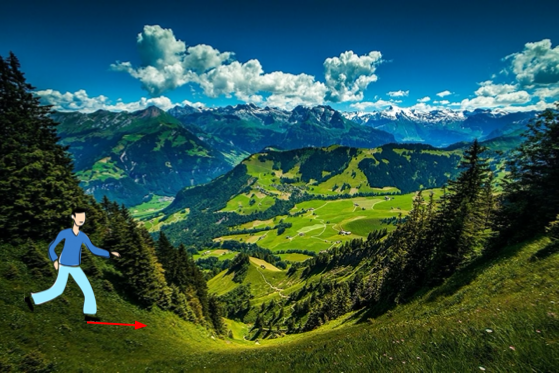
\includegraphics[height = 5cm, width=7cm]{figures/diag_GD.png} 
\end{figure}


\paragraph{A general approach:  line search method}
Given any initial guess $x_1$, the line search method uses the following algorithm
$$
\eta_t=\argmin_{\eta\in \mathbb{R}^1} f(x_t - \eta p_t)\qquad \mbox{\scriptsize(1D minimization problem)}
$$ 
 to produce $\{ x_{t}\}_{t=1}^{\infty}$
\begin{equation}\label{line-search}
x_{t+1} = x_{t} - \eta_t p_t.
\end{equation}
Here $\eta_t$ is called the step size in optimization and also learning
rate in machine learning, $p_t$ is called the descent direction, which
is the critical component of this algorithm. And $x_t$ tends to 
$$
x^*=\argmin_{x\in \mathbb{R}^n} f(x) \iff f(x^*)=\min_{x\in \mathbb{R}^n} f(x)
$$ 
as $t$ tends to infinity. There is a series of optimization
algorithms which follow the above form just using different choices of $p_t$.

Then, the next natural question is what a good choice of $p_t$ is? 
We have the following theorem to show why gradient direction is a good choice for $p_t$.
\begin{lemma}
Given  $x \in \mathbb{R}^n$, if $\nabla f(x)\neq 0$, the fast descent direction of $f$ at $x$ is the negative gradient direction, namely
\begin{equation}\label{key}
-\frac{\nabla f(x)}{\|\nabla f(x)\|} = \mathop{\arg\min}_{ p \in \mathbb{R}^n, \|p\|=1} \left. \frac{\partial f(x + \eta p)}{\partial \eta} \right|_{\eta=0}.
\end{equation}
It means that $f(x)$ decreases most rapidly along the negative gradient direction.
\end{lemma}
 
\begin{proof}
Let $p$ be a direction in $\mathbb{R}^{n},\|p\|=1$. Consider the local decrease of the function $f(\cdot)$ along direction $p$
$$
\Delta(p)=\lim _{\eta \downarrow 0} \frac{1}{\eta}\left(f(x+\eta p)-f(x)\right)=\left. \frac{\partial f(x + \eta p)}{\partial \eta} \right|_{\eta=0}.
$$
Note that 
\begin{equation}
\begin{split}
\left. \frac{\partial f(x + \eta p)}{\partial \eta} \right|_{\eta=0}=\sum_{i=1}^n\left. \frac{\partial f}{\partial x_i}(x + \eta p)p_i \right|_{\eta=0} =(\nabla f, p),
\end{split}
\end{equation}
which means that 
$$
f(x+\eta p)-f(x)=\eta(\nabla f(x), p)+o(\eta) .
$$ 
Therefore
$$
\Delta(p)=(\nabla f(x), p).
$$
Using the Cauchy-Schwarz inequality
$
-\|x\| \cdot\|y\| \leq( x, y) \leq\|x\| \cdot\|y\|,
$
we obtain 
$$
-\|\nabla f(x)\| \le (\nabla f(x), p)\le \|\nabla f(x)\| .
$$ 
Let us take
$$
\bar{p}=-\nabla f(x) /\|\nabla f(x)\|.
$$
Then
$$
\Delta(\bar{p})=-(\nabla f(x), \nabla f(x)) /\|\nabla f(x)\|=-\|\nabla f(x)\|.
$$
The direction $-\nabla f(x)$ (the antigradient) is the direction of the fastest local decrease of the function $f(\cdot)$ at point $x.$ 
\end{proof}

Here is a simple diagram for this property.
	\begin{figure}[H]
		\centering{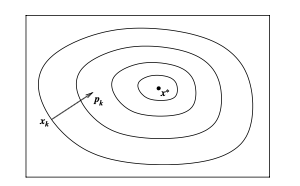
\includegraphics[width=5cm]{figures/gradientfast.png}}
		\caption{Negative Gradient Direction: $ x_t$ is current point, $ p_t$ is the negative gradient of $ x_t$, i.e., $- \nabla f( x_t)$.}
		\label{functiongradient}
	\end{figure}

Since at each point,  $f(x)$ decreases most rapidly along the negative
gradient direction, it is then natural to choose the search direction
in \eqref{line-search} in the negative gradient direction and the
resulting algorithm is the so-called gradient descent method.
\begin{algorithm}[H]
\caption{Gradient Descent Method} 
\label{alg:LR-R}
Given the initial guess $x_0$, learning rate $\eta_t>0$

	{\bf For} t=1,2,$\cdots$, \\
	\begin{equation}\label{key}
	x_{t+1} =  x_{t} - \eta_{t} \nabla f({x}_{t}), 
\end{equation}
\end{algorithm}

In practice, we need a ``stopping criterion'' that determines when the above gradient descent
method to stop.  One possibility is 
\begin{quote}
	{\bf While} $S(x_t; f) = \|\nabla f(x_t)\|\le \epsilon$ or $t \ge T$  
\end{quote}
for some small tolerance $\epsilon>0$ or maximal number of iterations
$T$.   In general, a good stopping criterion is hard to come by and it
is a subject that has called a lot of research in optimization for
machine learning. 

In the gradient method, the scalar factors for the gradients, $\eta_{t},$ are called the step sizes. Of course, they must be positive. There are many variants of the gradient method, which differ one from another by the step-size strategy. Let us consider the most important examples.
\begin{enumerate}
\item The sequence $\left\{\eta_t\right\}_{t=0}^{\infty}$ is chosen in advance. For example,
(constant step)
$$
\eta_t=\frac{\eta}{\sqrt{t+1}};
$$
\item Full relaxation:
$$
\eta_t=\arg \min _{\eta \geq 0} f\left(x_t-\eta \nabla f\left(x_t\right)\right);
$$
\item The Armijo rule: Find $x_{t+1}=x_t-\eta \nabla f\left(x_t\right)$ with $\eta>0$ such that
$$
\alpha\left(\nabla f\left(x_t\right), x_t-x_{t+1}\right) \leq f\left(x_t\right)-f\left(x_{t+1}\right),
$$
$$
\beta\left(\nabla f\left(x_t\right), x_t-x_{t+1}\right) \geq f\left(x_t\right)-f\left(x_{t+1}\right),
$$
where $0<\alpha<\beta<1$ are some fixed parameters.
\end{enumerate}
Comparing these strategies, we see that 
\begin{enumerate}
\item The first strategy is the simplest one. It is often used in the context of convex optimization. In this framework, the behavior of functions is much more predictable than in the general nonlinear case.
\item The second strategy is completely theoretical. It is never used in practice since even in one-dimensional case we cannot find the exact minimum in finite time.
\item The third strategy is used in the majority of practical algorithms. It has the following geometric interpretation. Let us fix $x \in \mathbb{R}^{n}$ assuming that $\nabla f(x) \neq 0$. Consider the following function of one variable:
$$
\phi (\eta)=f(x-\eta \nabla f(x)),\quad \eta\ge0.
$$
Then the step-size values acceptable for this strategy belong to the part of the graph of $\phi$ which is located between two linear functions:
$$
\phi_{1}(\eta)=f(x)-\alpha \eta\|\nabla f(x)\|^{2}, \quad \phi_{2}(\eta)=f(x)-\beta \eta\|\nabla f(x)\|^{2}
$$
Note that $\phi(0)=\phi_{1}(0)=\phi_{2}(0)$ and $\phi^{\prime}(0)<\phi_{2}^{\prime}(0)<\phi_{1}^{\prime}(0)<0 .$ Therefore, the
acceptable values exist unless $\phi(\cdot)$ is not bounded below. There are several very fast one-dimensional procedures for finding a point satisfying the Armijo conditions. However, their detailed description is not important for us now.
\end{enumerate}
